% 2
\section{類似研究}
VRとハンドジェスチャーを組み合わせる上で、作成したVRオブジェクトとセンサーで認識した物体情報の接触判定が重要となる。本研究では、二次元平面上の図形に対する内部外部判定を利用して、接触か非接触を判定する。そこで、二次元平面の図形の内部外部判定に関する研究を紹介する。

% 3.1
%\subsection{複雑形状認識の問題点と対処方法\cite{タグ2}}
%一般的に、複雑形状において内部外部判定を行う際には、外積計算による方法と、 Cauchy の積分定理による方法が用いられる。外積計算による方法の特徴としては、くぼみや穴などを有するドーナッツ型の図形に対する内部外部判定が困難である、というものが存在する。その一方で、複雑形状の図形において、境界線近くでの誤判定が比較的少ないというメリットが存在する。 Cauchy の積分定理による方法の特徴としては、くぼみや穴などを有するドーナッツ型の図形に対する内部外部判定が得意である、というものが存在する。一方で、複雑形状の図形において、境界線付近での判定に難があるというデメリットが存在する。従って、両判定方法を組み合わせることによって、より誤判定が少ない方法を提案することができる。



% 2.1
\subsection{Winding Number による内部外部判定\cite{タグ3}}
Winding Number というものを用いた内部外部判定方式が存在する。一般的に Winding Number Algorithm と呼ばれるものであるが、これは、内部外部判定したい点Pを中心に、多角形の辺を順番になぞる。この時、点Pの周りを何回回転するかを計算し、その値($wn$)によって内部か外部か判定する。$wn \geqq 1$ の際、多角形は点Pを取り囲んでいると判断できるため、点Pは多角形の内部であると判定される。$wn = 0$ の際、Pは多角形の外側であると判定される。

より具体的な方法を説明する。頂点 $V_0, V_1, \ldots, V_n (V_1 = V_n)$ からなる多角形Tにおいて、点Pと頂点 $V_i$ からなる線分 $L_i$、点Pと頂点 $V_{i+1}$ からなる線分 $L_{i+1}$ がなす角度の合計を考える(この角度は符号付きで、反時計回りを正、時計回りを負とする)。この時、 $\theta_i$ を $PV_i, PV_{i+1}$ のなす角度とすると、一回転は $2\pi$ より
\[
wn = \frac{1}{2\pi}\sum_{i=0}^{n-1}\theta_i
\]
となる。図2-1は、点が内部にある場合の例を示している。

\begin{center}
  \includegraphics[width=10cm]{wn_inside.eps} \\
 \vspace{1mm}
  図2-1. 点が内部に存在する場合
\end{center}

この時、$\theta_0, \ldots, \theta_4$ の合計を考えると、$2\pi$ になり、$wn = 1$ となることが分かる。従って、点Pは内部に存在すると判定される。図2-2は、点が外部にある場合の例を示している。

\begin{center}
  \includegraphics[width=10cm]{wn_outside.eps} \\
 \vspace{1mm}
  図2-2. 点が外部に存在する場合
\end{center}

この時、$\theta_0, \ldots, \theta_4$ の合計を考えると、$0$ になり、$wn = 0$ となることが分かる。従って、点Pは外部に存在すると判定される。この Winding Number Algorithm を使って、実際に内部外部判定を行ってみる。二次元のスクリーンを用意して、そこに図形の角を描画する。スクリーン上で、正方格子点を考えて、それぞれの格子点が図形の内部か外部かを判定する。結果は、図2-3のようになる。

 \vspace{-5mm}
\begin{center}
  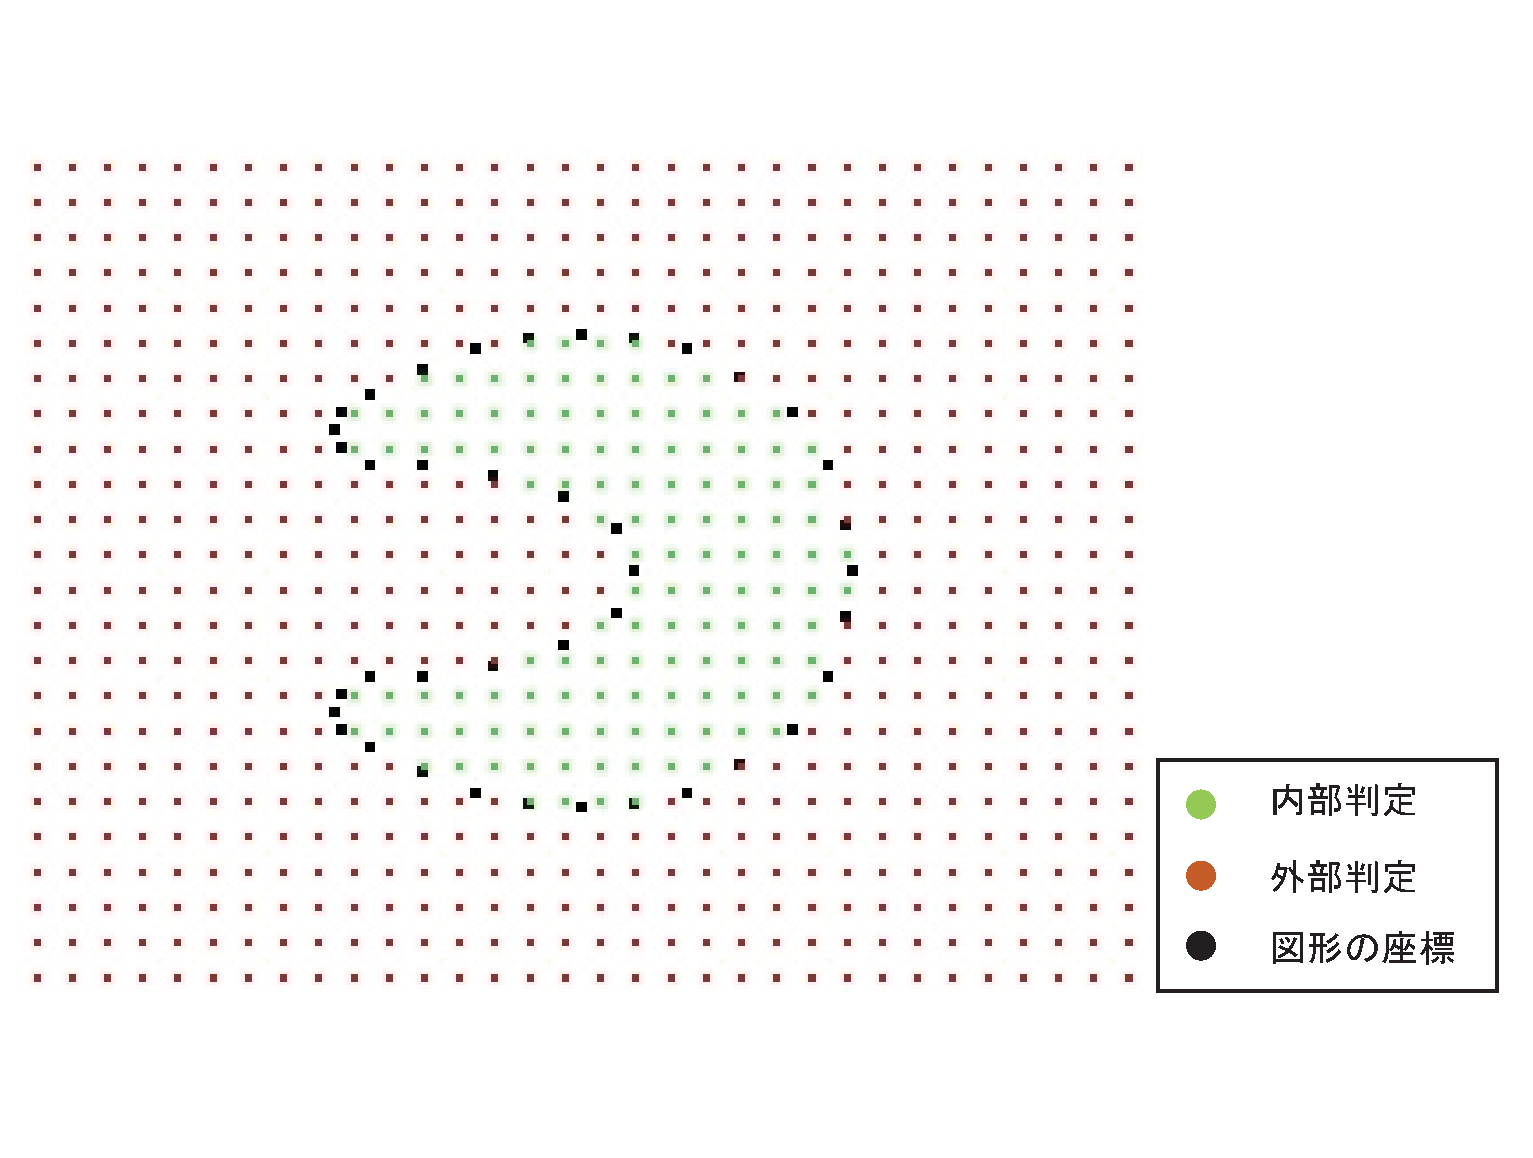
\includegraphics[width=14cm]{iedecision_2d.eps} \\
 \vspace{-10mm}
  図2-3. Winding Number Algorithm を用いた内部外部判定
\end{center}

一般に、$\theta = cos^{-1}(cos \theta), cos \theta = \frac{a \cdot b}{|a| \cdot |b|}$ より、
\[
wn = \frac{1}{2\pi}\sum_{i=0}^{n-1}cos^{-1}\left[\frac{(V_i - P) \cdot (V_{i+1} - P)}{|V_i - P||V_{i+1} - P|}\right]
\]
が成り立つ。この式より、内部外部判定を行えるが、三角関数 $cos^{-1} \theta$ を使用しているため、計算コストがかかる。















